%%big poster size with big fonts
\documentclass[extrafontsizes, 30pt]{memoir}
\usepackage[paperheight=31in,paperwidth=47in,margin=1in,heightrounded,showframe]{geometry}

%%background from pptx
\usepackage{background}
\backgroundsetup{
scale=1,
angle=0,
opacity=1,  %% adjust
contents={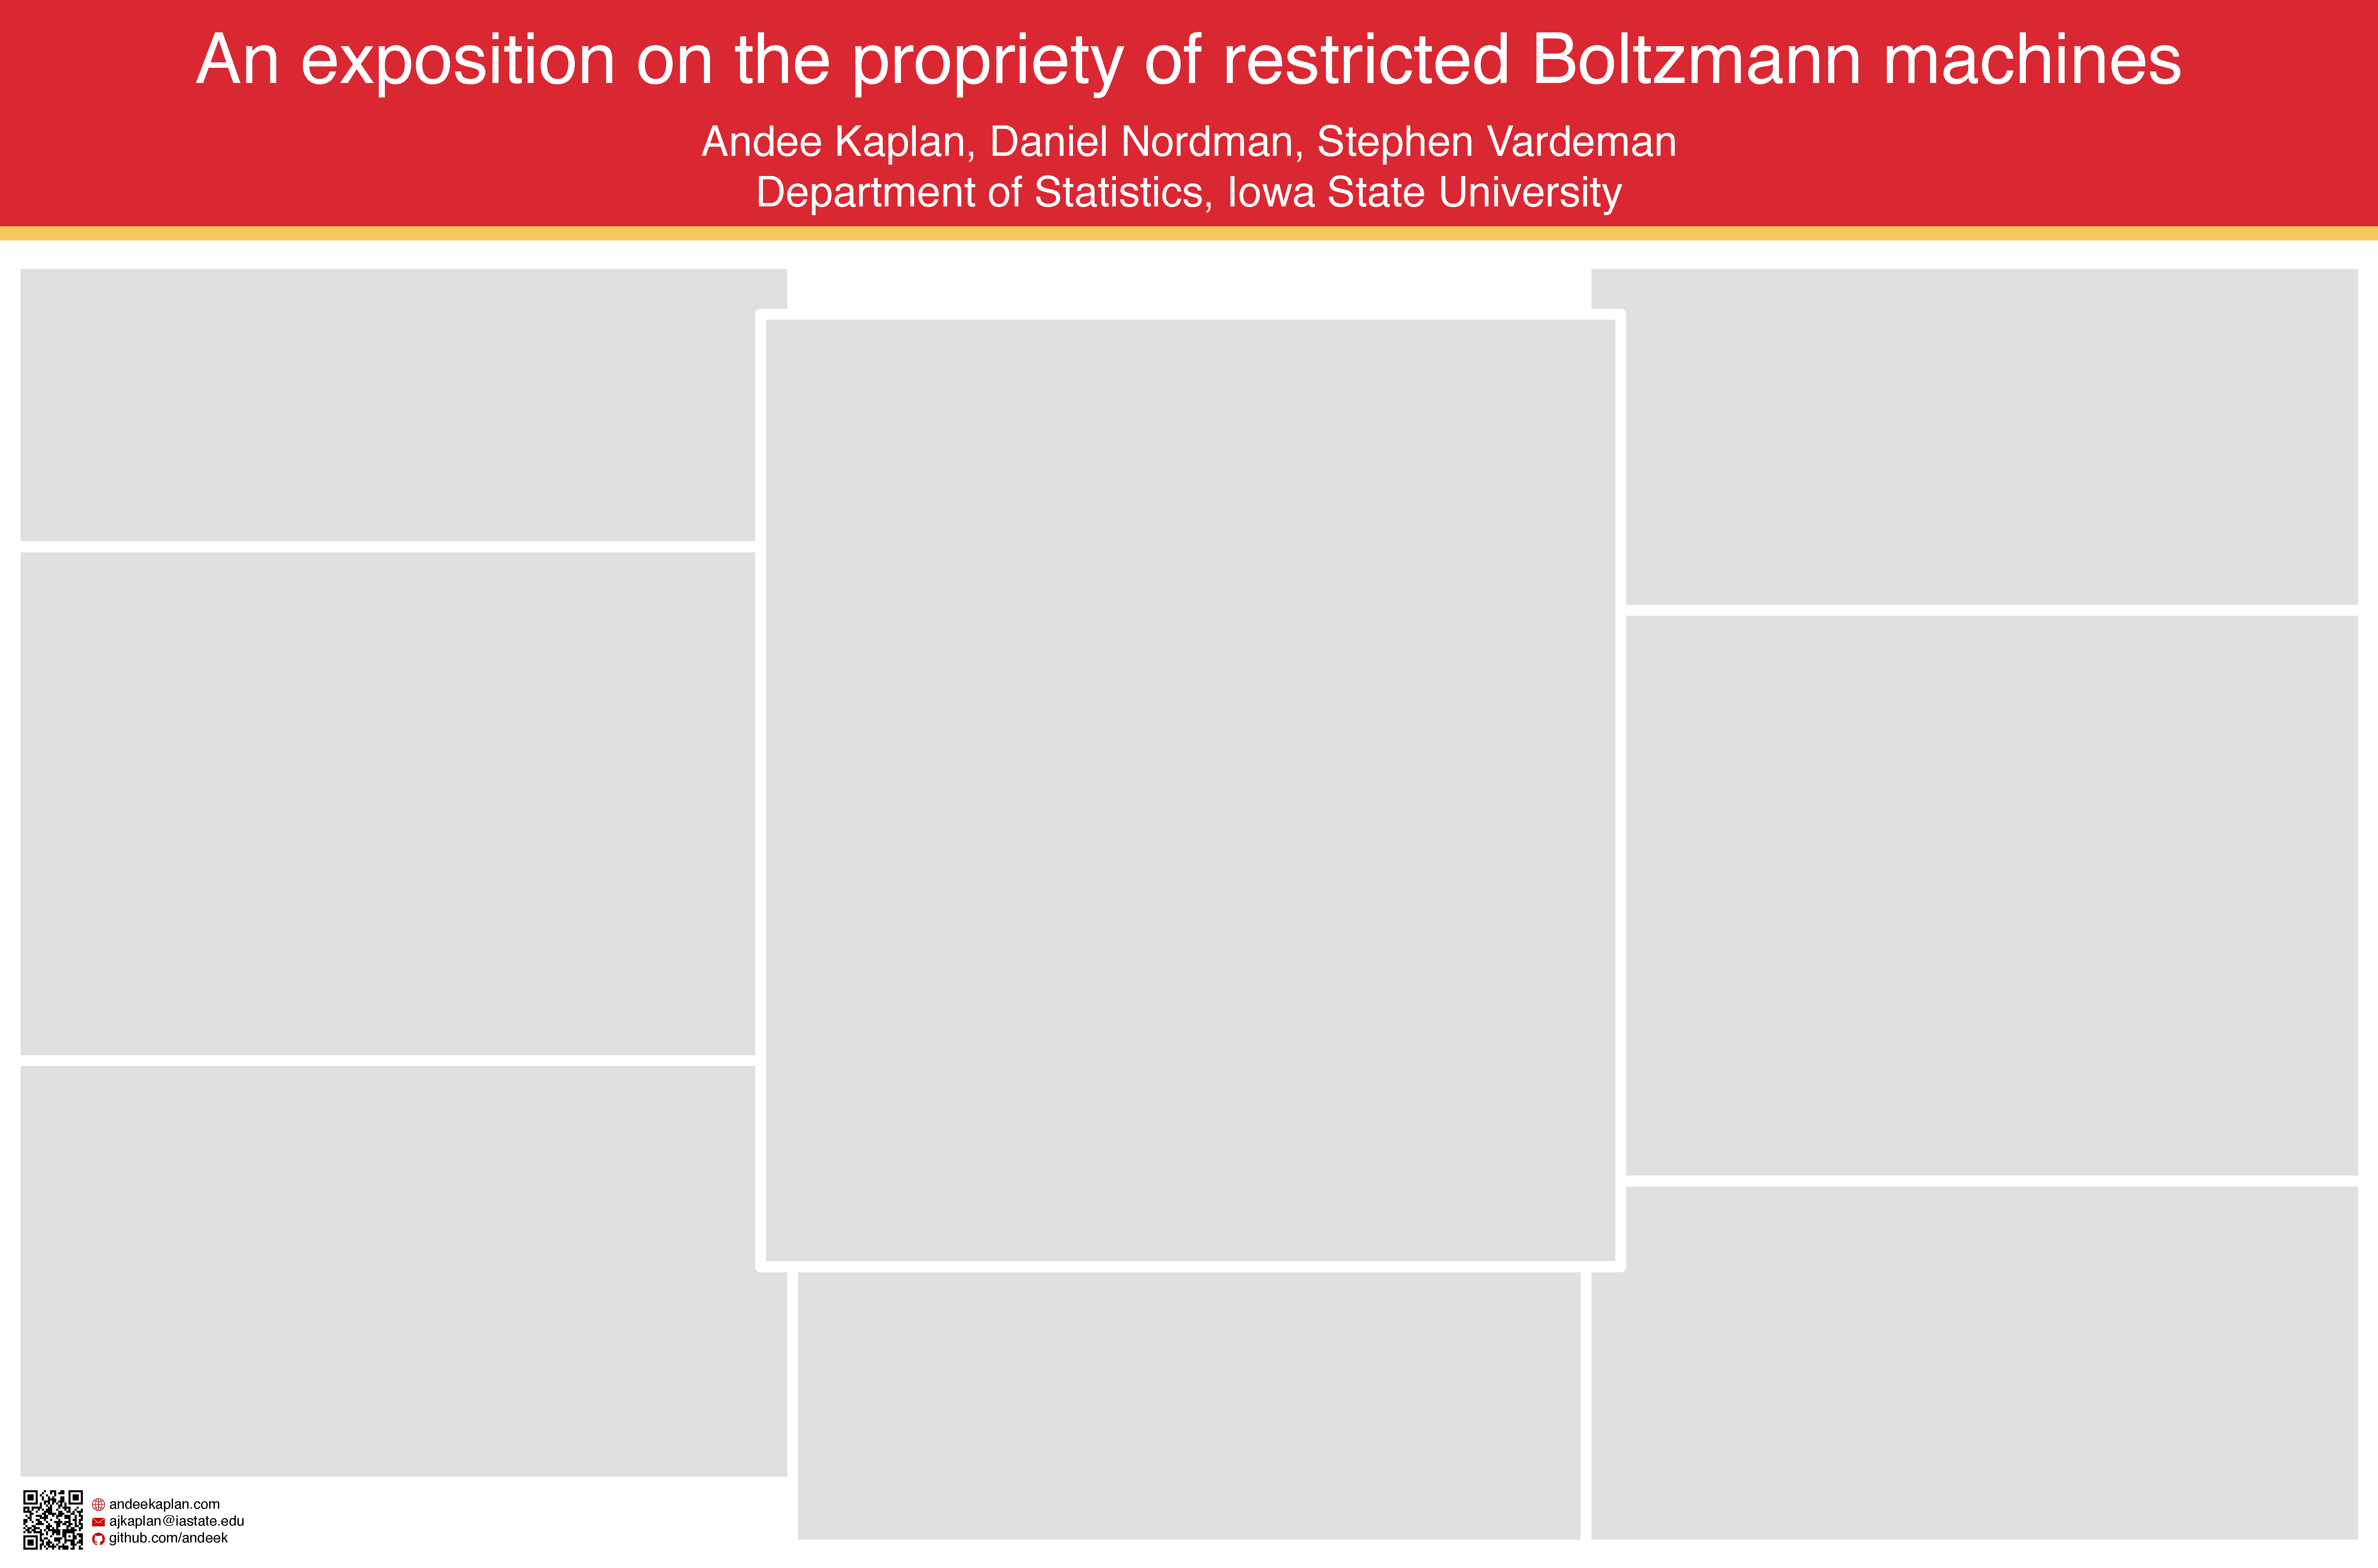
\includegraphics[width=\paperwidth,height=\paperheight]{images/coda2016_poster_background.pdf}}
}

%%put words where I want
\usepackage[absolute, overlay]{textpos}
\setlength{\TPHorizModule}{1in}
\setlength{\TPVertModule}{\TPHorizModule}

%%tikz setup
\usepackage{tikz, subfig, amsthm}
\usepackage{tikz-3dplot}
\usetikzlibrary{arrows, shapes, positioning}

%%other options
\definecolor{isublue}{RGB}{58,117,196}
\definecolor{isured}{RGB}{206,17,38}
\counterwithout{figure}{chapter}
\usepackage{amsmath}
\setlength{\parindent}{0cm}

\begin{document}

%%-----------------------------------------------
%%
%%Middle big box
%%
\begin{textblock}{18.01}(14.53, 6.71)
{\large \bfseries Restricted Boltzmann machine (RBM)}

\begin{figure}[ht]
  \centering
  \resizebox{\linewidth}{!}{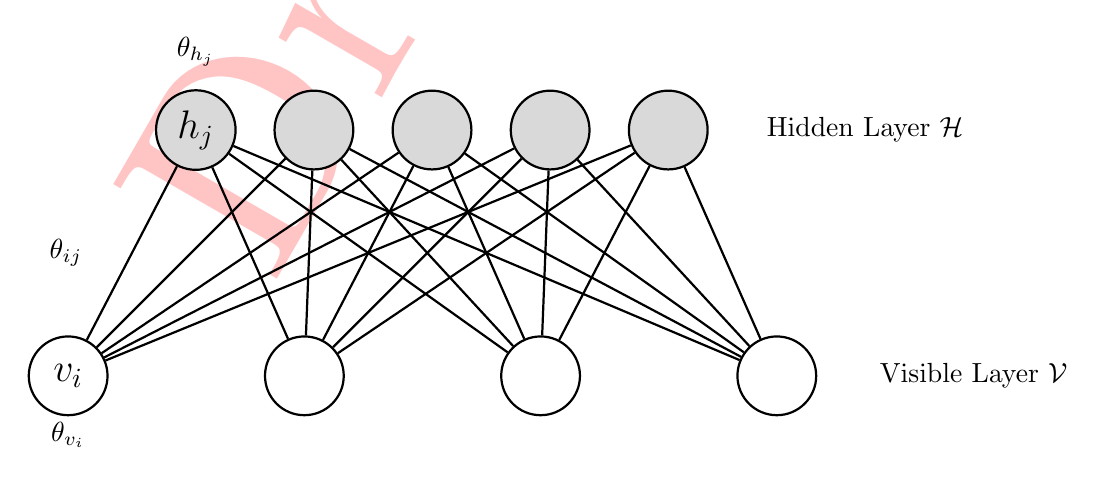
\begin{tikzpicture}[auto, node distance=3cm, thick, 
                    main node/.style= {circle,
                      fill=gray!30,
                      draw,
                      font=\sffamily\Large\bfseries,
                      minimum size=1cm}]
                      

  \node[main node] (1) {$h_j$};
  \node (11) [above of=1, yshift = -2cm] {$\theta_{h_j}$};
  \node[main node] (2) [right of=1, xshift = -1.5cm] {};
  \node[main node] (3) [right of=2, xshift = -1.5cm] {};
  \node[main node] (4) [right of=3, xshift = -1.5cm] {};
  \node[main node] (5) [right of=4, xshift = -1.5cm] {};
  \node (0) [right of=5, xshift = -.5cm] {Hidden Layer $\mathcal{H}$};
  \node[main node] (6) [below left of=1, fill=white, xshift = .5cm, yshift = -1cm] {$v_i$};
  \node (12) [below of=6, yshift = 2.25cm] {$\theta_{v_i}$};
  \node[main node] (7) [right of=6, fill=white] {};
  \node[main node] (8) [right of=7, fill=white] {};
  \node[main node] (9) [right of=8, fill=white] {};
  \node (10) [right of=9, xshift = -.5cm] {Visible Layer $\mathcal{V}$};
  
  \path
    (1) edge node [left=.5cm] {$\theta_{ij}$} (6)
        edge node {} (7)
        edge node {} (8)
        edge node {} (9)
    (2) edge node {} (6)
        edge node {} (7) 
        edge node {} (8)
        edge node {} (9)
    (3) edge node {} (6)
        edge node {} (7)
        edge node {} (8)
        edge node {} (9)
    (4) edge node {} (6)
        edge node {} (7) 
        edge node {} (8)
        edge node {} (9)
    (5) edge node {} (6)
        edge node {} (7) 
        edge node {} (8)
        edge node {} (9);
\end{tikzpicture}}
  \caption{An example restricted Boltzmann machine (RBM), which consists of two layers, a hidden ($\mathcal{H}$) and a visible layer ($\mathcal{V}$), with no connections within a layer. Hidden nodes indicated by gray circles and the visible nodes indicated by white circles.}
  \label{fig:rbm}
\end{figure}

\begin{figure}[ht]
  \centering
  \makeatletter
\pgfarrowsdeclare{latexnew}{latexnew}
{
  \ifdim\pgfgetarrowoptions{latexnew}=-1pt%
    \pgfutil@tempdima=0.28pt%
    \pgfutil@tempdimb=\pgflinewidth%
    \ifdim\pgfinnerlinewidth>0pt%
      \pgfmathsetlength\pgfutil@tempdimb{.6\pgflinewidth-.4*\pgfinnerlinewidth}%
    \fi%
    \advance\pgfutil@tempdima by.3\pgfutil@tempdimb%
  \else%
    \pgfutil@tempdima=\pgfgetarrowoptions{latexnew}%
    \divide\pgfutil@tempdima by 10%
  \fi%
  \pgfarrowsleftextend{+-1\pgfutil@tempdima}%
  \pgfarrowsrightextend{+9\pgfutil@tempdima}%
}
{
  \ifdim\pgfgetarrowoptions{latexnew}=-1pt%
    \pgfutil@tempdima=0.28pt%
    \pgfutil@tempdimb=\pgflinewidth%
    \ifdim\pgfinnerlinewidth>0pt%
      \pgfmathsetlength\pgfutil@tempdimb{.6\pgflinewidth-.4*\pgfinnerlinewidth}%
    \fi%
    \advance\pgfutil@tempdima by.3\pgfutil@tempdimb%
  \else%
    \pgfutil@tempdima=\pgfgetarrowoptions{latexnew}%
    \divide\pgfutil@tempdima by 10%
    \pgfsetlinewidth{0bp}%
  \fi%
  \pgfpathmoveto{\pgfqpoint{9\pgfutil@tempdima}{0pt}}
  \pgfpathcurveto
  {\pgfqpoint{6.3333\pgfutil@tempdima}{.5\pgfutil@tempdima}}
  {\pgfqpoint{2\pgfutil@tempdima}{2\pgfutil@tempdima}}
  {\pgfqpoint{-1\pgfutil@tempdima}{3.75\pgfutil@tempdima}}
  \pgfpathlineto{\pgfqpoint{-1\pgfutil@tempdima}{-3.75\pgfutil@tempdima}}
  \pgfpathcurveto
  {\pgfqpoint{2\pgfutil@tempdima}{-2\pgfutil@tempdima}}
  {\pgfqpoint{6.3333\pgfutil@tempdima}{-.5\pgfutil@tempdima}}
  {\pgfqpoint{9\pgfutil@tempdima}{0pt}}
  \pgfusepathqfill
}
\pgfsetarrowoptions{latexnew}{-1pt}
\pgfkeys{/tikz/.cd, arrowhead/.default=-1pt, arrowhead/.code={
  \pgfsetarrowoptions{latexnew}{#1}
}}

\begin{tikzpicture}[node distance=3cm, thick, 
                    visible/.style= {circle,
                      fill=isublue,
                      draw,
                      font=\Large,
                      inner sep=0pt,
                      minimum size=1cm},
                    hidden/.style= {circle,
                      fill=white,
                      draw,
                      font=\Large,
                      inner sep=0pt,
                      minimum size=1cm},
                    output/.style= {rectangle,
                    	fill=white,
                    	draw,
                    	font=\Large,
                    	inner sep=4pt,
                    	minimum size=1cm,
                    	rounded corners
                    },
                    classify/.style= {forbidden sign,
                    	fill=white,
                    	draw,
                    	font=\Large,
                    	inner sep=0pt,
                    	minimum size=2cm
                    },
                    remember picture]

    \node[anchor=north east,inner sep=0] (image) at (0,0) {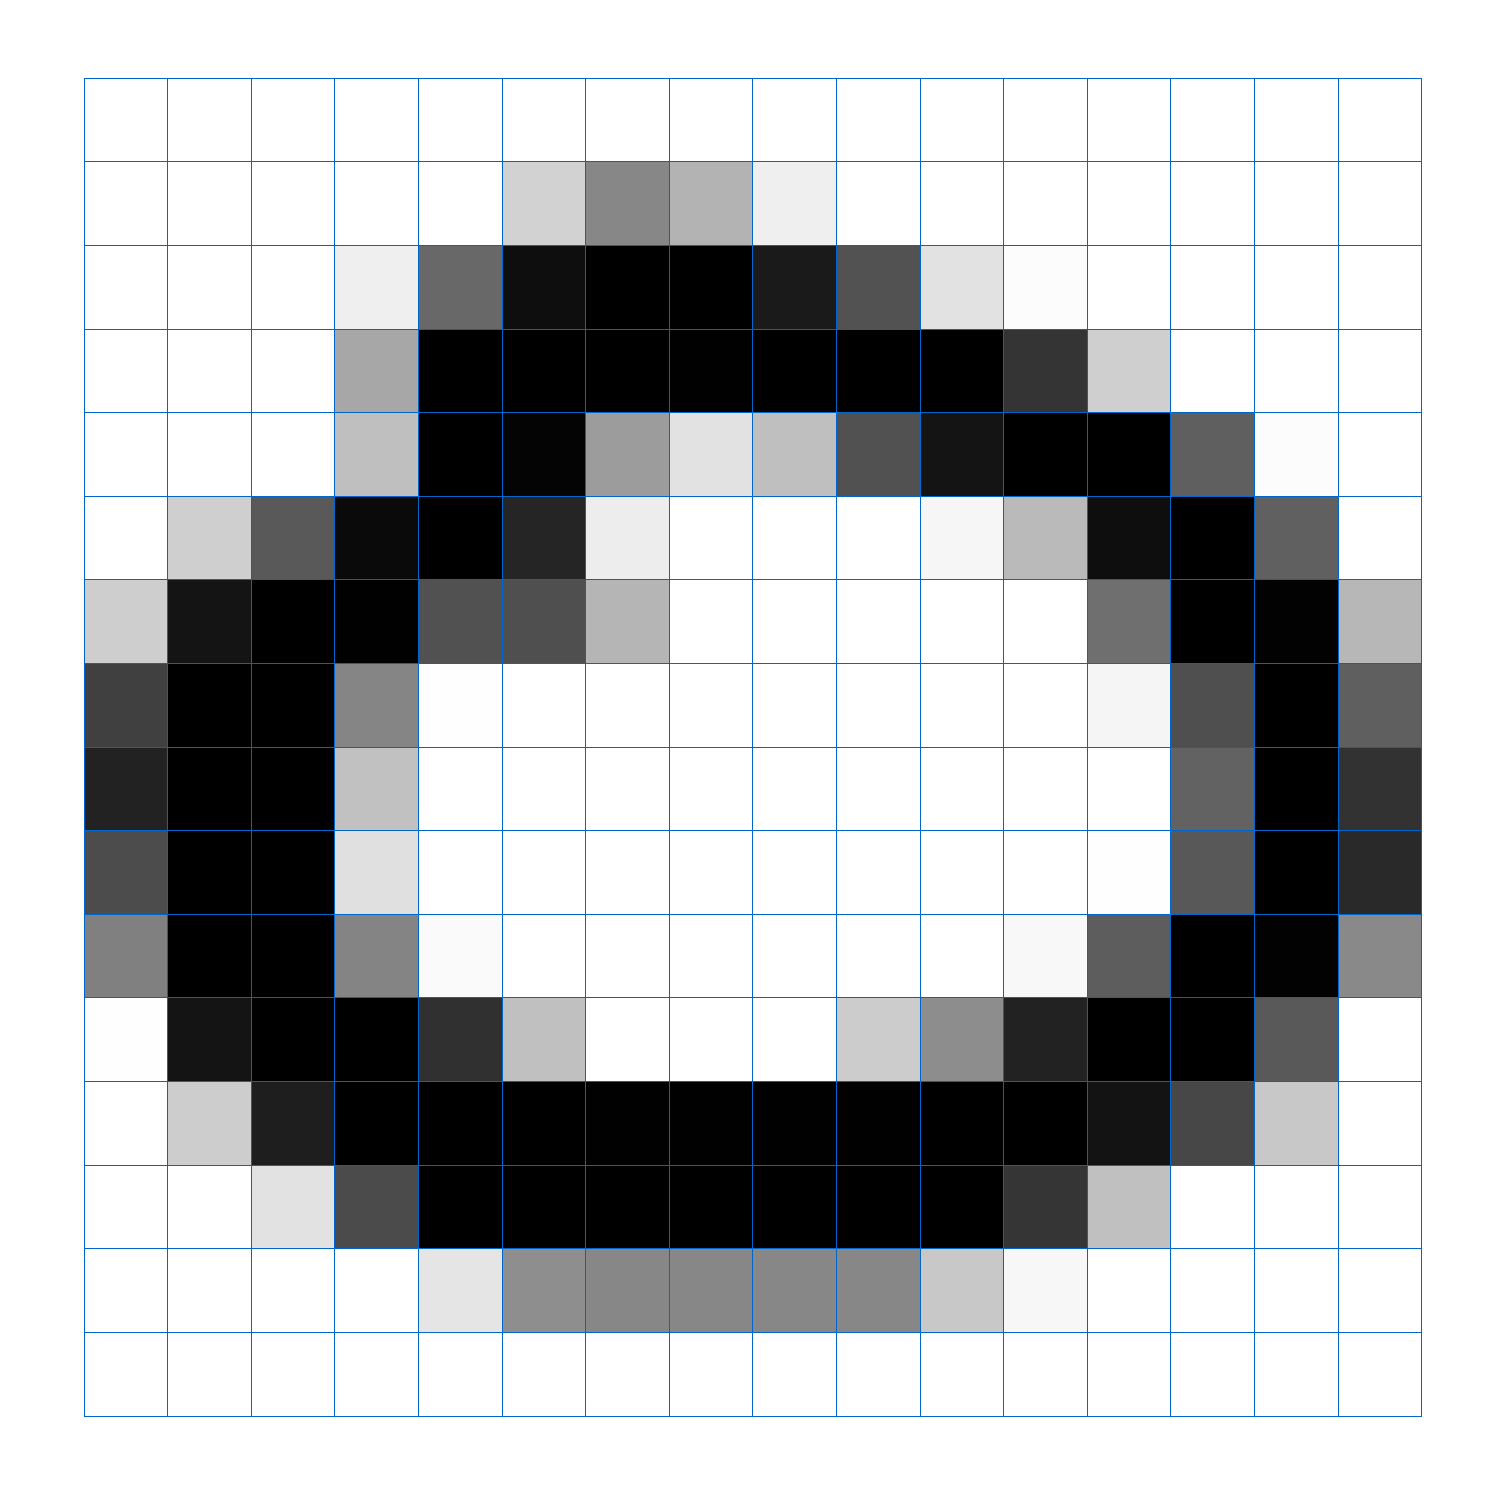
\includegraphics[height=2in]{visibles.pdf}};
    \begin{scope}[x={(image.south east)},y={(image.north west)}]
        \draw[isured, ultra thick] (0.05,0.05) rectangle (0.11,0.11);
    \end{scope}
    \node (11) [below of=image, font=\Large] {Example image};
    
	% define destination coordinates
	\path (-4.65,-.45) coordinate (first)
		  (-.45,-.45) coordinate (middle)
          (-.45,-4.65) coordinate (last);



    \node[visible] (1) [xshift = 2cm, yshift = -.8cm] {$v_1$};
    \node (2) [below of=1, yshift=2.25cm] {$\vdots$};
    \node[visible] (3) [below of=2, draw=isured, yshift=2cm] {$v_{16}$};
    \node (4) [below of=3, yshift=2.25cm] {$\vdots$};
    \node[visible] (5) [below of=4, yshift=2cm] {$v_{256}$};
    \node (12) [right of=11, xshift = 1.5cm, font=\Large] {$\mathcal{V}$};
    
    \node[hidden] (6) [right of=1] {$h_1$};
    \node(7)[below of=6, yshift=1.3cm] {$\vdotswide$};
    \node[hidden] (8) [right of=5] {$h_H$};
    %\draw [decorate, decoration={brace,amplitude=10pt}, xshift=-4pt,yshift=0pt](6,-.3) -- (6,-4.8) node (16) [black, midway, right=20pt] {};
    \draw[decoration={brace, raise=0pt, amplitude=10pt},decorate](6,-.3) -- node[right=0.5pt, midway] (16) {} (6,-4.8) ;
    
    \node (13) [right of=12, font=\Large] {$\mathcal{H}$};
    
    \node[output] (9) [right of=7, align = center, xshift=3cm] {Feature \\ representation};
    \node (14) [below of=9, font=\Large] {Output layer};
    \node[classify] (10) [right of=9, xshift=3cm, rotate=90] {};
    \node (15) [below of=10, font=\Large] {Classifier};
    
    \path
    (1) edge node {} (6)
        edge node {} (8)
    (3) edge node {} (6)
        edge node {} (8) 
    (5) edge node {} (6)
        edge node {} (8)
    (16) edge[-latexnew, arrowhead=.5cm] node {} (9)
    (9) edge[-latexnew, arrowhead=.5cm] node {} (10);
    
     \path[-latexnew, arrowhead=.5cm,black,thick] (first) edge (1);
     \path[-latexnew, arrowhead=.5cm,isured,thick] (middle) edge (3);
     \path[-latexnew, arrowhead=.5cm,black,thick] (last) edge (5);
\end{tikzpicture}

  \caption{Visibles diagram.}
  \label{fig:visibles}
\end{figure}

~\\[-1cm]
{\bfseries Joint distribution} \\[.25cm]
Let $\boldsymbol x = \{h_1, \dots, h_H, v_1,\dots,v_V\}$ represent the states of the visible and hidden nodes in an RBM. Then  the probability corresponding to the state of each node taking the value of $1$:
\begin{align}
\label{eqn:pmf}
f_{\boldsymbol \theta} (\boldsymbol x) = \dfrac{\exp\left(\sum\limits_{i = 1}^V \sum\limits_{j=1}^H \theta_{ij} v_i h_j + \sum\limits_{i = 1}^V\theta_{v_i} v_i + \sum\limits_{j = 1}^H\theta_{h_j} h_j\right)}{\sum\limits_{\boldsymbol x \in \mathcal{X}}\exp\left(\sum\limits_{i = 1}^V \sum\limits_{j=1}^H \theta_{ij} v_i h_j + \sum\limits_{i = 1}^V\theta_{v_i} v_i + \sum\limits_{j = 1}^H\theta_{h_j} h_j\right)} 
\end{align}
\end{textblock}

%%-----------------------------------------------
%%
%%Top left box
%%
\begin{textblock}{14.08}(.8, 5.71)
{\large \bfseries Deep learning}

\end{textblock}

%%-----------------------------------------------
%%
%%Middle left box
%%
\begin{textblock}{14.08}(.8, 11.83)
{\large \bfseries Degeneracy in random graph models}

\end{textblock}

%%-----------------------------------------------
%%
%%Bottom left box
%%
\begin{textblock}{14.08}(.8, 20.64)
{\large \bfseries Tiny example}

\end{textblock}

%%-----------------------------------------------
%%
%%Top right box
%%
\begin{textblock}{14.08}(33.5, 5.71)
{\large \bfseries Managable examples}
\end{textblock}

%%-----------------------------------------------
%%
%%Middle right box
%%
\begin{textblock}{14.08}(33.5, 12.91)
{\large \bfseries Fitting}

\end{textblock}

%%-----------------------------------------------
%%
%%Bottom right box
%%
\begin{textblock}{14.08}(33.5, 23.85)
{\large \bfseries Discussion}
\end{textblock}

%%-----------------------------------------------
%%
%%Bottom middle box
%%
\begin{textblock}{15.08}(16.17, 24.84)
{\large \bfseries References}
\end{textblock}

\end{document}